\section{Integration von ROS2 mit Zenoh} % (fold)
\label{sec:Integration von ROS2 mit Zenoh}

Wie im vorangegangenen Abschnitt beleuchtet, ist Zenoh ein wichtiger Baustein um die Brücke im \acrlong{cttc} zu schließen. Es nimmt die Rolle des Transportprotokolls für alle Teilnehmer im Kontinuum ein. Aus diesem Grund macht es Sinn, Zenoh in ROS2 einzubinden um die Roboter in das Kontinuum zu integrieren.\\
Aus dieser Motivation heraus, wird in diesem Abschnitt die Integration von ROS2 mit Zenoh erläutert. Dabei wird zu Beginn auf die generellen Gründe hinter der Nutzung von Zenoh im Robotics Bereich eingegangen. Schließlich, wird die Technische Implementation beschrieben und die Nutzung im \acrlong{cttc} erläutert.\\

Die Nutzung von Zenoh in ROS2 hat viele positive Auswirkungen auf die Kommunikation zwischen den Robotern. Neben der bereits erwähnten Einbindung in das \acrlong{cttc}, bietet Zenoh eine Reihe von Vorteilen gegenüber dem standard Kommunikationsservice in ROS2, dem \acrlong{dds}.\\

Ein Hauptgrund Zenoh zu nutzen ist das ineffiziente Discovery Protokoll vom \acrlong{dds}. Dieses wurde mit kabelgebundenen Architekturen im Hinterkopf entworfen und kommt bei modernen Kabellosen Architekturen an ihre Grenzen. Erkennen lässt es sich am großen overhead, welches das DDS Discovery Protokoll im Vergleich zu Zenoh im Netzwerk erzeugt \cite{ZenohZeroOverhead2022}. Der Grund für die Ineffizienz beim austauschen der Daten ist die Funktionsweise des Discovery Mechanismus. Bei einem falsch konfigurierten Netz sendet der Discovery Mechanismus dabei immer weitere Suchanfragen aus und kann das Netz massiv überlasten. ROS2 ging dieses Problem an, in dem es einen neuen Discovery Server \cite{DiscoveryServerSettings} einführte der das Netzwerk Overhead verringert. Doch wie im Namen enthalten, wird hier ein neuer, zentraler Server gebraucht der die Discovery unterstützt. Dies macht es wiederrum für viele Peer-To-Peer Anwendungsfälle schwer nutzbar. Zenoh wiederrum, bietet ohne zentralen Server ebenfalls eine gute Discovery Performance. Im Gegensatz zu dem Discovery Mechanismus in DDS, nutzt Zenoh das Konzept der "Resource Generalisation"\cite{ZenohZeroOverhead2022}. Dabei kann das Protokoll je nach Einstellung nur ein Bruchteil der Daten übertragen die vom Netzwerk für die Entdeckung der Services gebraucht werden. Bei einem Roboter der folgende Datenquellen published:
\begin{enumerate}
  \item Temperatur: \code{/robot1/sensor/temperatue}
  \item Druck: \code{/robot1/sensor/pressure}
  \item Orientierung: \code{/robot1/dynamics/odometry}
\end{enumerate}

Kann der Zenoh Router 'Ressource Generalisation' anwenden, in dem es nur die Daten \code{/robot1/sensor/**} und \code{/robot1/dynamics/**} oder \code{/,robot1/**} im Discovery Mechanismus weitergibt. Dadurch kann die Datenmenge in einer Anfrage komprimiert werden und das Netzwerk besser skalieren. Dies ist wichtig , wenn man beispielsweise über das Internet mit sehr vielen Clients skalieren möchte.\\
Das Zweite Argument für die Nutzung von Zenoh als Kommunikationsprotokoll ist die Skalierbarkeit im Bezug auf das \acrlong{cttc}. Das Ziel ist wie im Eingangskapitel erwähnt, die Skalierung auf Ebene des Internets. Durch den bereits erwähnten Discovery Mechanismus von DDS, stößt man hier jedoch an Grenzen. Neben dem bereits erwähnten Problem des Netzwerk Overheads, bringt es weitere Nachteile im Kontext der Skalierung mit. Roboter die sich in weiteren Subnetzen befinden, können nicht automatisch gefunden werden. Daraus ergibt sich ein Problem wenn man über das Internet Skalieren möchte. Da vor allem letzteres ein wichtiger Grundpfeiler beim \acrlong{cttc} ist, lohnt es sich eine Integration mit Zenoh einzubauen.\\

Außer den genannten Gründen, macht die Unterstützung von leistungsschwachen Robotern in einem Umfeld instabiler Verbindungen das Zenoh Protokoll interessant für die Robotik. Zum einen braucht man keine Rücksicht auf die Leistung verschiedener Roboter nehmen und kann sich auf den jeweiligen Use case konzentrieren den man erreichen möchte. Zum anderen kann Zenoh mit instabilen Verbindungen gut umgehen. Grund dafür ist die Konstruktion der Verbindungen zwischen den Teilnehmern in einem Zenoh Netzwerk. Dabei werden bei einer Zenoh Verbindung zwei Arten von Kanälen aufgebaut \cite{Eclipsezenoh}. Der eine Kanal ist auf Zuverlässigkeit getrimmt. Der andere arbeitet nach dem \textit{Best Effort} Prinzip und kann nicht zwangsläufig eine fehlerfreie Übermittlung garantieren. Dabei ist es möglich zuverlässige Kanäle zwischen zwei Teilnehmern zu erstellen die mehrere Hops dazwischen haben. Das ist Sinnvoll, wenn die Zuverlässigkeit eine hohe Priorität hat. Zusätzlich kümmert sich das Protokoll um die Fragmentierung und die maximale Nutzung der vorhandenen Verbindung um möglichst effizient zu arbeiten.\\

Zusammenfassend ist die Einbindung von Zenoh in ROS2 eine große Hilfe um die Robotik mit den Zielen des \acrlong{cttc} zu vereinen und das in \ref{sub:Cloud-To-Thing-Continuum} vorgestellte Konzept des Robot-to-anything (R2X) zu erreichen. Es tut dies, in dem es viele Defizite von DDS ausgleicht und die Skalierbarkeit entlang des \acrlong{cttc} möglich macht.\\

\subsection{Einbindung von Zenoh im Data Distribution Service} % (fold)
\label{sub:Einbindung von Zenoh im Data Distribution Service}

Nachdem die Motivation für die Nutzung von Zenoh in ROS2 erläutert wurde, wird nun auf die technische Implementierung eingegangen. Diese basiert auf einen leichtgewichtigen Übersetzer zwischen dem ROS2 Roboter und einem weiteren Zenoh Client. Das Ziel ist dabei die transparente Überführung von DDS-Nachrichten in einen für das Zenoh Protokoll geeignetes Format. Mit diesem, ist es dann möglich Nachrichten zwischen verschiedenen Zenoh Knoten auszutauschen. Diese können weitere ROS2 Instanzen oder Server an der Edge oder Cloud sein.\\

Um externe Services an Zenoh anzubinden werden Plugins genutzt. Diese bilden die Brücke zwischen den verschiedenen Systemen. Im Fall von ROS2 wird eine Brücke zwischen dem \acrlong{dds} und dem Zenoh Protokoll gebraucht. Das Zenoh DDS Plugin erfüllt diese Aufgabe und ist als Open Source Projekt auf GitHub zu finden \cite{Eclipsezenoh}.\\
Um Nachrichten an das Zenoh Protokoll weiterzuleiten, erkennt das Plugin die vom \acrlong{dds} bereitgestellten Entities und generiert ein jeweiliges Paar für Zenoh.

\begin{figure}
  \begin{center}
    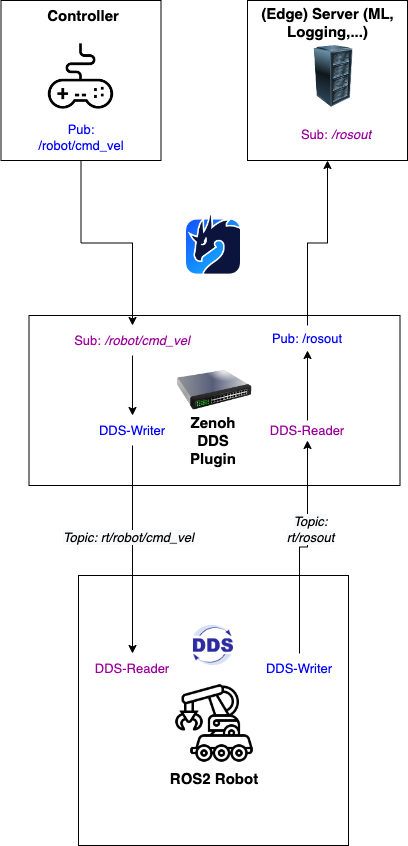
\includegraphics[width=0.5\textwidth]{figures/ros2-dds.drawio.png}
  \end{center}
  \caption{ROS2 DDS Plugin}
  \label{fig:ros2-dds}
\end{figure}

Das Beispiel in Abbildung \ref{fig:ros2-dds} zeigt die Funktionsweise in einer vereinfachten Form. Auf dem ROS2 Roboter gibt es dabei ein DDS-Reader und ein DDS-Writer. Der Reader hört auf das Topic \code{rt/robot/cmd\_vel} und bekommt hier Informationen um seine Geschwindigkeit anzupassen. Der DDS-Writer published dabei allgemeine ROS Informationen auf dem Topic \code{rt/rosout}.\\
Um das Zenoh Protokoll anzubinden kommt jetzt das Zenoh DDS Plugin zum Einsatz. Dieses findet automatisch die vom DDS Angebotenen Reader und Writer. Daraufhin erstellt er für jeden der Topics einen dazugehörigen DDS-Reader oder Writer. Für einen Reader, einen Writer und umgekehrt. Dies lässt sich an \ref{fig:ros2-dds} in der ersten Verbindung erkennen. Nützlich ist auch, dass das Plugin die in \ref{sub:Einbindung von Zenoh im Data Distribution Service} angesprochenen Quality-of-Service Policies ebenfalls übernimmt. Schlussendlich erstellt das Plugin für jeden Reader einen Zenoh Subscriber und für jeden Writer einen Zenoh Publisher mit dem der Roboter nun an das Zenoh Netzwerk eingebunden wäre. In dem betrachteten Beispiel gibt es noch einen Controller der die Robotersteuerung übernimmt und ein Server der die Log Daten aus dem Roboter speichert.

% subsection Einbindung von Zenoh im \acrlong{dds} (end)

% section sec:Integration von ROS2 mit Zenoh (end)
